% Created by tikzDevice version 0.12.3.1 on 2022-07-27 15:26:40
% !TEX encoding = UTF-8 Unicode
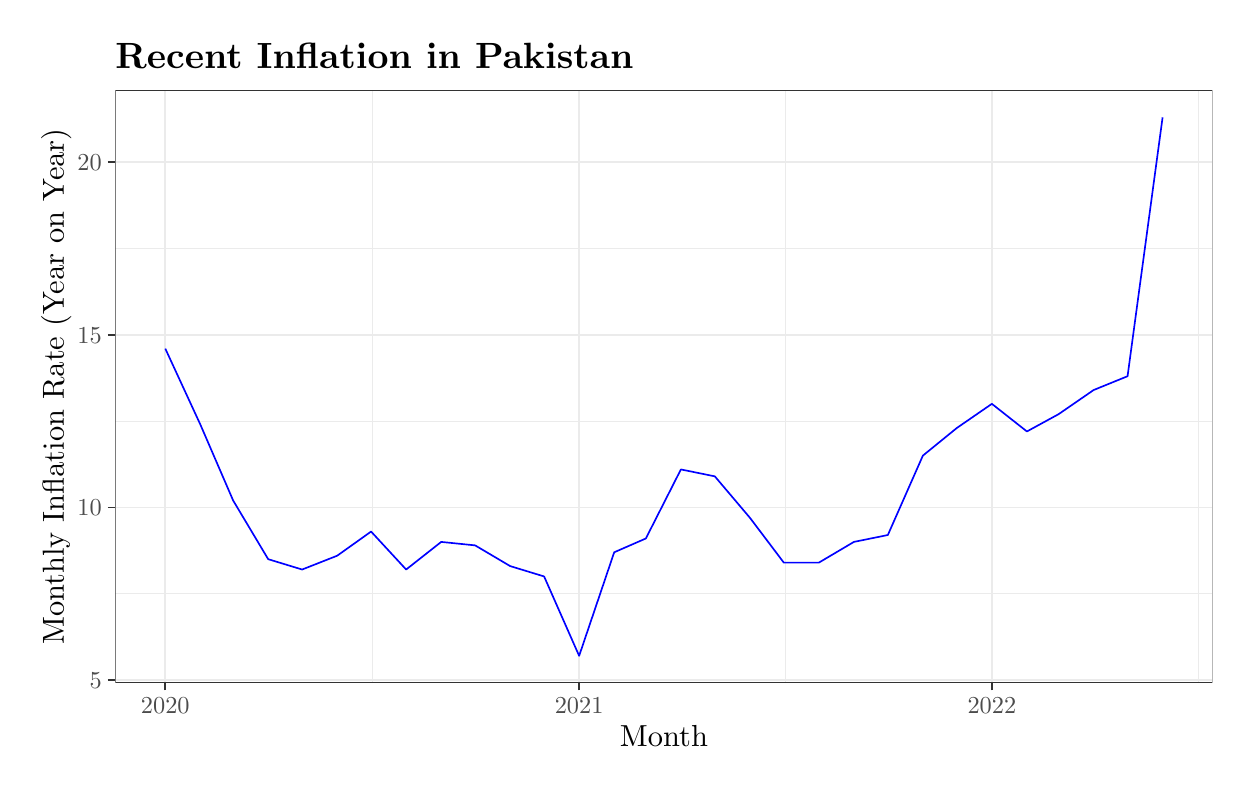
\begin{tikzpicture}[x=1pt,y=1pt]
\definecolor{fillColor}{RGB}{255,255,255}
\path[use as bounding box,fill=fillColor,fill opacity=0.00] (0,0) rectangle (433.62,267.40);
\begin{scope}
\path[clip] (  0.00,  0.00) rectangle (433.62,267.40);
\definecolor{drawColor}{RGB}{255,255,255}
\definecolor{fillColor}{RGB}{255,255,255}

\path[draw=drawColor,line width= 0.6pt,line join=round,line cap=round,fill=fillColor] (  0.00,  0.00) rectangle (433.62,267.40);
\end{scope}
\begin{scope}
\path[clip] ( 31.71, 30.69) rectangle (428.12,244.72);
\definecolor{fillColor}{RGB}{255,255,255}

\path[fill=fillColor] ( 31.71, 30.69) rectangle (428.12,244.72);
\definecolor{drawColor}{gray}{0.92}

\path[draw=drawColor,line width= 0.3pt,line join=round] ( 31.71, 62.87) --
	(428.12, 62.87);

\path[draw=drawColor,line width= 0.3pt,line join=round] ( 31.71,125.23) --
	(428.12,125.23);

\path[draw=drawColor,line width= 0.3pt,line join=round] ( 31.71,187.60) --
	(428.12,187.60);

\path[draw=drawColor,line width= 0.3pt,line join=round] (124.50, 30.69) --
	(124.50,244.72);

\path[draw=drawColor,line width= 0.3pt,line join=round] (273.84, 30.69) --
	(273.84,244.72);

\path[draw=drawColor,line width= 0.3pt,line join=round] (423.18, 30.69) --
	(423.18,244.72);

\path[draw=drawColor,line width= 0.6pt,line join=round] ( 31.71, 31.68) --
	(428.12, 31.68);

\path[draw=drawColor,line width= 0.6pt,line join=round] ( 31.71, 94.05) --
	(428.12, 94.05);

\path[draw=drawColor,line width= 0.6pt,line join=round] ( 31.71,156.41) --
	(428.12,156.41);

\path[draw=drawColor,line width= 0.6pt,line join=round] ( 31.71,218.78) --
	(428.12,218.78);

\path[draw=drawColor,line width= 0.6pt,line join=round] ( 49.73, 30.69) --
	( 49.73,244.72);

\path[draw=drawColor,line width= 0.6pt,line join=round] (199.27, 30.69) --
	(199.27,244.72);

\path[draw=drawColor,line width= 0.6pt,line join=round] (348.41, 30.69) --
	(348.41,244.72);
\definecolor{drawColor}{RGB}{0,0,255}

\path[draw=drawColor,line width= 0.6pt,line join=round] ( 49.73,151.43) --
	( 62.40,123.98) --
	( 74.25, 96.54) --
	( 86.91, 75.34) --
	( 99.17, 71.60) --
	(111.84, 76.59) --
	(124.09, 85.32) --
	(136.76, 71.60) --
	(149.43, 81.58) --
	(161.68, 80.33) --
	(174.35, 72.84) --
	(186.61, 69.10) --
	(199.27, 40.41) --
	(211.94, 77.83) --
	(223.38, 82.82) --
	(236.04,107.77) --
	(248.30,105.27) --
	(260.97, 90.31) --
	(273.23, 74.09) --
	(285.89, 74.09) --
	(298.56, 81.58) --
	(310.82, 84.07) --
	(323.48,112.76) --
	(335.74,122.74) --
	(348.41,131.47) --
	(361.07,121.49) --
	(372.51,127.73) --
	(385.18,136.46) --
	(397.44,141.45) --
	(410.10,234.99);
\definecolor{drawColor}{gray}{0.20}

\path[draw=drawColor,line width= 0.6pt,line join=round,line cap=round] ( 31.71, 30.69) rectangle (428.12,244.72);
\end{scope}
\begin{scope}
\path[clip] (  0.00,  0.00) rectangle (433.62,267.40);
\definecolor{drawColor}{gray}{0.30}

\node[text=drawColor,anchor=base east,inner sep=0pt, outer sep=0pt, scale=  0.88] at ( 26.76, 28.65) {5};

\node[text=drawColor,anchor=base east,inner sep=0pt, outer sep=0pt, scale=  0.88] at ( 26.76, 91.02) {10};

\node[text=drawColor,anchor=base east,inner sep=0pt, outer sep=0pt, scale=  0.88] at ( 26.76,153.38) {15};

\node[text=drawColor,anchor=base east,inner sep=0pt, outer sep=0pt, scale=  0.88] at ( 26.76,215.75) {20};
\end{scope}
\begin{scope}
\path[clip] (  0.00,  0.00) rectangle (433.62,267.40);
\definecolor{drawColor}{gray}{0.20}

\path[draw=drawColor,line width= 0.6pt,line join=round] ( 28.96, 31.68) --
	( 31.71, 31.68);

\path[draw=drawColor,line width= 0.6pt,line join=round] ( 28.96, 94.05) --
	( 31.71, 94.05);

\path[draw=drawColor,line width= 0.6pt,line join=round] ( 28.96,156.41) --
	( 31.71,156.41);

\path[draw=drawColor,line width= 0.6pt,line join=round] ( 28.96,218.78) --
	( 31.71,218.78);
\end{scope}
\begin{scope}
\path[clip] (  0.00,  0.00) rectangle (433.62,267.40);
\definecolor{drawColor}{gray}{0.20}

\path[draw=drawColor,line width= 0.6pt,line join=round] ( 49.73, 27.94) --
	( 49.73, 30.69);

\path[draw=drawColor,line width= 0.6pt,line join=round] (199.27, 27.94) --
	(199.27, 30.69);

\path[draw=drawColor,line width= 0.6pt,line join=round] (348.41, 27.94) --
	(348.41, 30.69);
\end{scope}
\begin{scope}
\path[clip] (  0.00,  0.00) rectangle (433.62,267.40);
\definecolor{drawColor}{gray}{0.30}

\node[text=drawColor,anchor=base,inner sep=0pt, outer sep=0pt, scale=  0.88] at ( 49.73, 19.68) {2020};

\node[text=drawColor,anchor=base,inner sep=0pt, outer sep=0pt, scale=  0.88] at (199.27, 19.68) {2021};

\node[text=drawColor,anchor=base,inner sep=0pt, outer sep=0pt, scale=  0.88] at (348.41, 19.68) {2022};
\end{scope}
\begin{scope}
\path[clip] (  0.00,  0.00) rectangle (433.62,267.40);
\definecolor{drawColor}{RGB}{0,0,0}

\node[text=drawColor,anchor=base,inner sep=0pt, outer sep=0pt, scale=  1.10] at (229.92,  7.64) {Month};
\end{scope}
\begin{scope}
\path[clip] (  0.00,  0.00) rectangle (433.62,267.40);
\definecolor{drawColor}{RGB}{0,0,0}

\node[text=drawColor,rotate= 90.00,anchor=base,inner sep=0pt, outer sep=0pt, scale=  1.10] at ( 13.08,137.70) {Monthly Inflation Rate (Year on Year)};
\end{scope}
\begin{scope}
\path[clip] (  0.00,  0.00) rectangle (433.62,267.40);
\definecolor{drawColor}{RGB}{0,0,0}

\node[text=drawColor,anchor=base west,inner sep=0pt, outer sep=0pt, scale=  1.32] at ( 31.71,252.79) {\bfseries Recent Inflation in Pakistan};
\end{scope}
\end{tikzpicture}
